This chapter describes first the overall structure of the project, its technical requirements (which can and later be used as part of the evaluation) and then dives into the implementation of individual modules.

I refer to this project by its name \textsl{graffs}.
A working version is published on GitHub\footnote{\url{https://github.com/jjurm/graffs}} along with its source code.


\section{Overview}

The purpose of this project is to develop a methodology and tool, i.e. a framework, to help study graph metrics, and empirically analyse their robustness in particular.

\begin{figure}[p!]
    \centering
    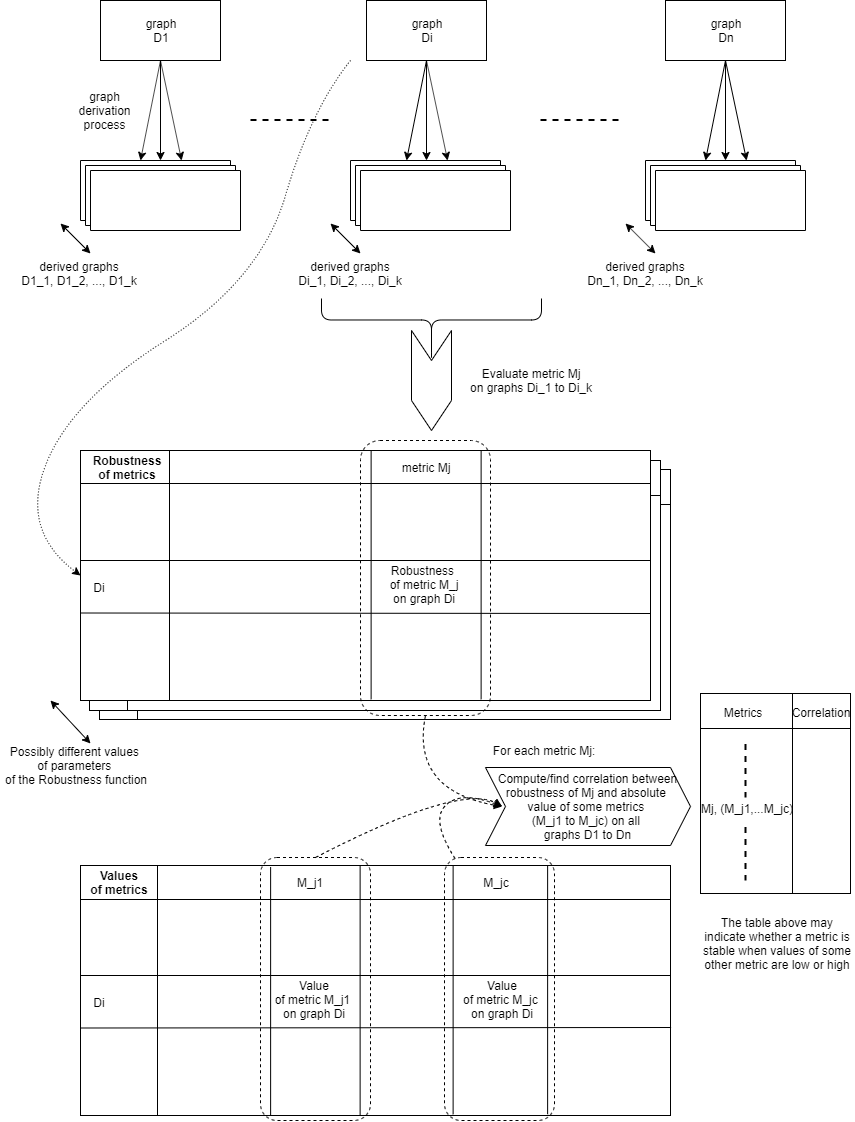
\includegraphics[width=16cm]{proposal_diagram1.png}
    \caption{An illustration of the evaluation process.\\ \todo{make this diagram up to date, using notation from~\nameref{ch:preparation}}.
    A generator is used to generate perturbed graphs from each input dataset.
    Each metric from a chosen set of metrics is evaluated on all petrurbed graphs.
    From those results, robustness values of each metric on each dataset are calculated using each chosen robustness measures.
    This is referred to in the project as the ``Main pipeline''}
    \label{fig:overview_prop_diagram}
\end{figure}


\graffs is a command-line tool written in Kotlin\citeneeded that can load/store datasets of different formats, generate perturbed graphs, evaluate metrics, and calculate robustness values. \autoref{fig:overview_prop_diagram} is a diagram explaining the natural flow of the program, i.e. the \textsl{main pipeline} where we start with graph datasets and end up with deductions about each metric's robustness.


\section{Design goals}\label{sec:design-goals}

The following are technical requirements I set for the project.
Overall, I aim this tool to be reusable for similar projects, either by directly invoking the compiled binary, or by using it as a dependency, or by forking and extending it.

\subsection{Supported features}

\graffs supports the following features:

\begin{enumerate}
    \item Store, load input graphs in various formats, and represent them in a unified memory structure
    \item Run algorithms that compute metrics on graphs
    \item Generate graphs by applying perturbations to given input graphs
    \item Run experiments by evaluating metrics on generated graphs in a systematic manner
    \item Calculate robustness of metrics based on experiments
    \item Possibly, produce visual output from the results
\end{enumerate}

\subsection{Scalability}

According to The Paper~\cite{Bozhilova2019}, calculating natural connectivity for a single node for a graph with ~7000 nodes takes ~88 seconds on a standard computer.
In one of my toy examples, calculating average betweenness centrality of ~2500 nodes took ~8 minutes on my personal computer.
Thus, assuming computing a (computation-heavy) metric(s) on an input graph of average size 5000 nodes takes ~30 minutes, the pure computation time suggested by the~\nameref{ch:proposal} would take the following time on a standard personal computer (approximated in the order of magnitude)
\[(\sim 6\ \text{datasets}) \times (\sim 6\ \text{metrics}) \times (\sim 50\ \text{derived graphs}) \times (\sim 30\ \text{minutes}) \approx 38\ \text{days}\]

For this reason, one of the goals is to make the program efficient and runnable on a supercomputer, utilising the power of multi-core systems for parallel execution.

\subsection{Reproducibility}

It is important for all results in research to be reproducible.
By \textsl{reproducibility} of \graffs I mean the guarantee that one can exactly reproduce any results produced by the program.
I.e. when the program is run two times with the same input and hyper-parameters, it must produce the same output.
And by \textsl{the same output} I mean producing the same images, tables, numbers up to a bit-wise match.

This is a challenge in all the following areas:
\begin{itemize}
    \item \textbf{Stochastic processes}

    Methods based on stochastic processes or randomness must be reproducible.
    An example of a stochastic method are graph generators.

    These can be made reproducible done by generating all randomness starting off with a given seed for the generator.

    \item \textbf{Resolving ties}

    Methods that are not inherently stochastic but require pseudo-randomness to resolve ties must also be reproducible.
    An example is generating a visual layout for graphs such as in \autoref{fig:simple_graph}.
    This layout algorithm needs to resolve ties when starting with a graph where nodes have no position.

    Again, a solution is to base such flow on an input seed.

    \item \textbf{External factors}

    Unpredictability introduced by the operating system and other external factors must be accounted for, so that the program still produces the same results even if run on a different supported machine, in a different environment.
    This is more challenging in a concurrent environment when it must be made sure the produced output does not depend on any factors such as uncertainty and unpredictability of the OS's thread scheduler.

    These issues are resolved using a robust programming language and concurrency synchronisation approaches.
\end{itemize}

\subsection{Flexibility}

The program must be flexible enough, in particular the following:
\begin{enumerate}
    \item Usable on all widely used machines and operating systems
    \item Accepting input datasets (and any input parameters) in common formats
    \item As a library, it must provide modular access to individual parts of the program, so that it is easy to use \graffs as a dependency in future projects of a similar kind
\end{enumerate}


\section{Architecture}

In this section I explain major decisions about the platform.

\todo{Work In Progress from here below...}


\subsection{Kotlin language}

I used the programming language \textbf{Kotlin}, mainly for the following reasons.
It is by nature similar to Java and can be used together with other Java code in a single project.
Performance-wise, Kotlin is comparable to Java.
\begin{itemize}
    \item Concise, reducing the amount of boilerplate code
    \item Safer, preventing a significant number of errors
    \item IDE-friendly, allowing the IDE to help with software engineering
    \item Allows more functional constructs than Java
    \item Compiles to Java byte code and so preserves other important benefits of Java: Object-Oriented, platform-independent, extensible.
\end{itemize}

Using Kotlin in the project still allows including any libraries written in Java, as Kotlin compiles the \texttt{.kt} files to Java-bytecode \texttt{.class} files.

\todo{diagram of Kotlin, Gradle, Git, server}

\subsection{Version Control System}

The source code of the \graffs tool is stored in a Git repository, which keeps track of all code changes and allows understanding how code changed over time as well as restoring previous versions.

The repository can be found at \url{https://github.com/jjurm/graffs}.

\subsection{Build automation}

The project uses Gradle\citeneeded for project management.
Split into different modules, Gradle also helps to keep the structure well defined and manages builds of each module separately (which is called a multi-project build in Gradle).

Project configuration rules are set up using the \texttt{build.gradle} files (one in the root directory, then one within each module) with a number of plugins to facilitate the following and more:
\begin{enumerate}
    \item Defines the structure of the project, such as the directories for each module, and source and build directories of each
    \item Automates the process of compiling the code, running tests and producing deployable \texttt{jar}s
    \item Manages and automatically downloads dependencies
    \item Helps with version numbering
    \item Generates HTML API documentation for Kotlin and Java classes
\end{enumerate}


\todo{maybe put all subsections below somewhere at the end of Implementation}



\subsection{Remote computing cluster}

I used a remote computing facility provided by the Systems Research Group (\url{https://www.cl.cam.ac.uk/research/srg/}), sponsored by Dr Andrew Moore (\url{andrew.moore@cl.cam.ac.uk}).

In particular, I worked with the server \texttt{rio.cl.cam.ac.uk} with \todo{include computing characteristics}.

\subsubsection{Setting up the cluster}



\subsection{Project modules}

The project is structured in the following modules, using multi-project builds in Gradle:
\begin{itemize}
    \item \texttt{core} - APIs for structures, metrics, generators, etc., as well as the core data model for storing data in the database
    \item \texttt{storage} - accessing and loading graphs/datasets stored in the filesystem
    \item \texttt{generators} - graph generators
    \item \texttt{metrics} - graph metrics
    \item \texttt{robustness} - robustness measures
    \item \texttt{cli} - code for command-line interface
\end{itemize}

\todo{diagram of code structure + modules + packages}


\section{Main pipeline}


\subsection{Data model}




\subsubsection{Java Persistence API}

\subsubsection{Entities}
\begin{enumerate}
    \item GeneratedGraph
    \item MetricExperiment
\end{enumerate}

\subsubsection{Database}

\subsubsubsection{Storing graphs in database}

For evaluation of robustness, we need to be able to compare either values or ranks of values of a specific node between two generated graphs, therefore we need to be able to preserve mapping of nodes of a generated graph to nodes in the original dataset.
Thus, a node ID originating from the original dataset must be stored, not just values of a metric for each node.

I considered the following formats of storing graph:
\begin{enumerate}
    \item DGS
    \item DOT - doesn't preserve node IDs
\end{enumerate}


\subsection{Loading graphs}

\subsubsection{Edge files}

\subsubsection{RData files}


\subsection{Generating graphs}

\todo{work in progress}

For evaluating robustness of graph metrics according to the model described in the~\nameref{ch:proposal}, we need to evaluate graph metrics on a number of similar graphs - graphs that all describe the same facts from the real world.
We need to be able compare value of a metric between different graphs that \textit{share the same source} or are \textit{of the same foundation}.

One specific example may be a graph constructed from social network, such as Facebook.
Let $G_0$ be a dataset constructed from people and their mutual friendships at Facebook, and let $G_1$ be a graph constructed from people, with the set of edges including only stronger friendships. $G_0$ and $G_1$ have the same nodes, but edges of $G_1$ is a subset of edges of $G_0$.
Now, $G_0, G_1$ are different but describe the same structure of people in the world, i.e.\ convey the same meaning.

\textbf{Preserving node identities} For two such graphs, we can define subsets $V_{c0}$ and $V_{c1}$ of nodes of the respective graphs, such that there exists a bijection $V_{c0} \leftrightarrow V_{c1}$.
These nodes will have important meaning for definition of the robustness function, because the pairs of corresponding nodes describe the same entities of the real world.
Thus, we can observe how a graph metric behaves for a particular node in different graphs.


\subsubsection{Random edge deletion}

\subsubsection{Thresholding edges of protein graphs}


\subsection{Evaluating metrics}


\subsection{Metric robustness}


\subsection{Visualising graphs}


\section{Parallelism using Kotlin coroutines}

\section{Command line interface}

\todo{hierarchical diagram of nested command groups and their options}



\section{Testing}

\subsection{Unit testing}
Using JUnit 5

\subsection{Continuous Integration}
CircleCI


\section{Documentation}

The Kotlin code is documented using the \texttt{KDoc} language and an HTML documentation is generated using the \texttt{Dokka} tool (similar to \texttt{JavaDoc}).\citeneeded

I wrote the documentation in code most thoroughly for public classes, and their members that need clarification on their behaviour or usage.



